\documentclass[DIV=13,fontsize=11pt]{scrartcl}
\usepackage[T1]{fontenc}
\usepackage{lmodern}
\usepackage[ngerman]{babel}
\usepackage[utf8]{inputenc}
\usepackage{csquotes}
\usepackage[hidelinks]{hyperref}
\usepackage{amsmath}
\usepackage{amssymb} 
\usepackage{listings}
\usepackage{float}
\usepackage{dirtree}
\usepackage{booktabs}
\usepackage{graphics,graphicx}
\usepackage[left=2cm, right=2cm, top=2cm, bottom=2cm, bindingoffset=1cm, includeheadfoot]{geometry}
\usepackage[onehalfspacing]{setspace}
\usepackage[backend=biber,style=numeric,maxcitenames=1,sorting=none]{biblatex}\addbibresource{bib.bib}

% aendert u.a. bei zitierungen zu et al.
\DefineBibliographyStrings{ngerman}{ 
   andothers = {et\addabbrvspace al\adddot},
   andmore   = {et\addabbrvspace al\adddot},
}

\setlength{\parindent}{0pt}

\begin{document}
% ----------------------------------------------------------------------------
\subject{Projektbericht zum Modul Data Mining Wintersemester 20221/2022}
\title{Reproduktion des Papers \\ \textit{Context-Sensitive Visualization of Deep Learning Natural Language Processing Models}\cite{dunn2021context}}
\author{Max Henze}% obligatorisch
\maketitle% verwendet die zuvor gemachte Angaben zur Gestaltung eines Titels
% ----------------------------------------------------------------------------

\section{Einleitung}
% Beitrag Originalartikel: bessere Visualisierung von Wortwichtigkeit bei Klassifizierung durch Transformer Neural Network
% bearbeitete Teile: alle ( LNO Algorithmus und zusätzlich eigenes BERT Modell) 
% neue Erkenntnisse: 
% eigener Beitrag: Code zum Originalartikel, da keiner vorhanden 

Neuronale Netzwerke sind ein beliebtes Hilfmittel im Bereich von NLP.
Besonderst Modelle, welche sich den Einsatz von Transformern zur Hilfe nehmen,
wie BERT~\cite{devlin2018bert} oder GPT-2~\cite{radford2019language},
gehören schon lange zum state-of-the-art. Doch diese Modelle mit ihrer
Vielzahl an Layern, Neuronen und Verbindungen, gewähren einen nicht
gerade einfachen Einblick in ihre Verarbeitungsschritte.
\citeauthor{dunn2021context} haben daher in ihrem Artikel \citetitle{dunn2021context}
eine Methode entwickelt um Wörter, mit ihrer unterschiedlichen Wichtigkeitsgewichtung
innerhalb der Klassifizierung, zu visualisieren.
Als Replikationsziele wurden für diese Arbeit der gesamte Visualisierungsprozess
von \citeauthor{dunn2021context} gewählt. Zusätzlich dazu wurde ein eigenes
BERT Modell auf dem gegebenen IMDB~\cite{maas-EtAl:2011:ACL-HLT2011} trainiert um
dieses für den späteren Klassifikationsprozess zu verwenden.
Durch die Replikation wird eine verständliche Codebeigabe zum Originalartikel
erzeugt, welche dem Leser ein noch besseres Verständnis liefern soll. So können
mit dem System alle Dokumente des Testdatensatzes klassifiziert und visualisiert werden
um so eine größere Vielfalt von Beispielen bereitzustellen.

\section{Umfang der Replikation/Reproduktion}
% Behauptung/Hypothese: bessere Visualisierung von Wortwichtigkeit durch leve-n-out mit abhängigen Wörtern

Als Ziel dieser Replikation wurde die einzige Hypothese gewählt, welche
\citeauthor{dunn2021context} in ihrem Artikel behandeln. Sie propagieren,
dass sich die Wichtigkeit eines Wortes innerhalb der Klassifikation durch ein
Neuronales Netzwerk nicht nur durch den Vergleich der sogenannten
Prediction Strength (Sicherheit des NN, dass Label richtig Klassifiziert)
des Originaltextes zur Pediction Strength des Textes ohne das betrachtete Wort (leave-one-out)
ergibt, sondern dass der Einbezug von kontextuell zusammhängenden Wörtern (leave-n-out)
ebenfalls wichtig ist. \glqq Unser Ansatz schaut auf die Kombination von
Wörtern und Sätzen um deren Einfluss auf die Ausgabe des Modells zu erkennen,
was zu einer Visualisierung führt, welche kontextsensitiver zum Originaltext ist.
\grqq~\cite{dunn2021context}\\

Somit ist folgende Behauptung das Ziel dieser Replikation:

\begin{itemize}
    \item Leave-n-out Ansatz ist effektiver bei der Erkennung wichtiger Wörter als leave-one-out.
\end{itemize}

\section{Methoden}

Die Replikation des Originalartikels ergibt sich wie folgt. Durch die
fehlende Beigabe von Code mussten alle Ideen und Modelle von \citeauthor{dunn2021context}
eigenständig implementiert werden. Dazu wurde sich an Wortangaben
der Autoren wie zum Beispiel:
\glqq Der gesamte Code ist geschrieben in Python 3.8 und nutzt die Tensorflow Version
der Transformersbilbiothek. [...] Texttokenisierung und Abhängigkeitsbestimmung wurden
mit der spaCy NLP Bibliothek durchgeführt.\grqq~\cite{dunn2021context}\\

Zur Klassifizierung von Dokumenten wurde ein Modell unter der Verwendung von BERT trainiert.
Da keine weitere Angaben zu finden waren und eine große Auswahl an unterschiedlichen
BERT Modellen zu finden ist wurde das \textit{BERT uncased L-12 H-768 A-12} Modell gewählt,
welches auf Tensorflow Hub\footnote{\url{https://tfhub.dev}} zu den am häufigsten verwendet
BERT Modellen zählt.\\

Entwickelt wurde innerhalb eines Jupyter Notebooks mit Python.
Die folgenden essentiellen Packages fanden dabei Anwendung:

\begin{figure}[H]
    \centering
    \begin{tabular}{ll}
        \toprule
        Package Name    & Package Funktion                             \\
        \midrule
        tensorflow\_hub & Einbindung des BERT Modells                  \\
        tensorflow      & Modellerzeugung und Training                 \\
        official.nlp    & Trainingsoptimisierung                       \\
        spacy           & Abhängigkeitsbestimmung (Dependency Parsing) \\
        pandas          & Arbeiten mit Dataframes                      \\
        matplotlib      & Visualisierung der Texte                     \\
        \bottomrule
    \end{tabular}
    \caption{Verwendete Packages}
    \label{fig:packages}
\end{figure}

Zusätzlich wurde das BERT Modell auf einer Nvidia Geforce RTX 3070 mit 8 GB Arbeitsspeicher
trainiert.

\subsection{Modellbeschreibung}

Innerhalb des Originalartikels sind keine Angaben bezüglich der Zielfunktion und
Parameter zu finden. Angaben zum Modell beruhen auf der Benennung eines BERT Modells und
einer Modellbeschreibung, welche auf das Anhängen eines Dropout-Layers und
Dense-Layers verweist.\\

Die beschriebene Methodik ist wie folgt:\\

Ein Text wird durch das Modell klassifiziert und die damit korrespondierende
Ausgabestärke wird notiert. Nun werden mit Hilfe einer Abhängigkeitsbestimmung
alle Beziehungen zwischen Wörtern aufgedeckt. Anschließend werden neue Texte
erzeugt, in denen jeweils ein Wortpaar, welches eine Verbindung zueinander
aufweist, entfernt wurde. Die nun erhaltene Sammlung an neuen Texten wird wieder
durch das Modell klassifiziert und die neuen Ausgabestärken werden mit der
des Ausgangstextes verglichen. Texte mit größeren oder gleichen Ausgabestärken
als der des Originals tragen scheinbar nicht zur Klassifikation bei und werden
entfernt. Je größer die Differenz umso wichtiger war das
Wortpaar für die Klassifizierung. Mit Hilfe einer Linearisierung der Differenzen
und einer Colormap können Wörter smomit bezüglich ihrer Wichtigkeit
farblich kenntlich gemacht werden. Je wichtiger umso grüner, je unwichiger, desto blauer.

\subsection{Datenbeschreibung}

\begin{figure}[H]
    \centering
    \begin{minipage}{5cm}
        \dirtree{%
            .1 data.
            .2 test.
            .3 neg.
            .4 x\_y.txt.
            .4 ....
            .3 pos.
            .4 x\_y.txt.
            .4 ....
            .2 train.
            .3 neg.
            .4 x\_y.txt.
            .4 ....
            .3 pos.
            .4 x\_y.txt.
            .4 ....
        }
    \end{minipage}
    \caption{Ordnerstruktur des Datensatzes. x ist die Dokumentenid und y ist eine Sternewertung von Null bis Zehn.}
    \label{fig:filestruc}
\end{figure}

Der im Originalartikel und dieser Replikation verwendete Datensatz ist das Large Movie
Review Dataset~\cite{maas-EtAl:2011:ACL-HLT2011} der Universität Stanford.
Dieser umfasst 50.000 Dokumente, darunter 25.000 Trainingsdokumente und 25.000 Testdokumente. Er ist unter
\url{https://ai.stanford.edu/~amaas/data/sentiment/} verfügbar.\\

Der Datensatz hat eine vorgegebene Ordnerstruktur, siehe Abbilung \ref{fig:filestruc}.
So befinden sich die Trainingsdokumente und Testdokumente in eigenen Ordnern,
wobei positive und negative Dokumente nochmals in eigene Ordner unterteilt sind.
Die Dokumente unterscheiden sich stark in der Länge, so gibt es Dokumente mit knapp über 50 Zeichen
aber auch solche mit über 13.000 Zeichen.
Die Dokumente an sich sind nicht aufbereitet, enthalten englische Altagssprache und Sonderzeichen.

\begin{figure}[H]
    \centering
    \begin{lstlisting}
        Fair drama/love story movie that focuses on the lives of 
        blue collar people finding new life thru new love.The acting 
        here is good but the film fails in cinematography,screenplay,
        directing and editing.The story/script is only average at best.
        This film will be enjoyed by Fonda and De Niro fans and by 
        people who love middle age love stories where in the coartship 
        is on a more wiser and cautious level.
        It would also be interesting for people who are 
        interested on the subject matter regarding illiteracy.......
    \end{lstlisting}
    \caption{Beispieltext eines positiven Trainingsdokuments}
\end{figure}

Bei der Verwendung der Daten zum Training des Modells, wurde der Trainingsdatensatz zusätzlich in einen
Validierungsdatensatz aufgeteilt. Dieser umfasst 20 Prozent der Trainingsdaten und somit 5.000 Dokumente.

\subsection{Hyperparameter}

Folgende Hyperparameter wurden gesetzt:

\begin{figure}[H]
    \centering
    \begin{tabular}{ll}
        \toprule
        Parameter    & Wert \\
        \midrule
        Batch Size   & 16   \\
        Epochs       & 1    \\
        Learningrate & 3e-5 \\
        \bottomrule
    \end{tabular}
\end{figure}

Die Batch Size definiert die Menge an Trainingsdaten, welche von Netzwerk aufeinmal
verarbeitet werden bevor es sich updated. Diese wurde auf 16 festgesetzt, da das
Training auf der zuvor schon erwähnten Nvidia Grafikkarte trainiert werden sollte.
Größere Batch Sizes haben sich als Problem entpuppt, da diese nicht mehr in den
Speicher passten.
Bei der Epochenanzahl wurde nur eine festgelegt.
Beginnend lag dieser Wert bei fünf. Doch unterschiedliche Werte und eine Einbindung
von Early Stopping ergaben, dass das Modell nach der ersten Epoche die
beste Leistung aufwies. Mit zunehmenden Training stieg auf dem Trainingsdatensatz
die Accuracy und im selben Moment sank der Loss. Doch auf dem Validierungsdatensatz
stieg der Loss bei gleichbleibener Accuracy in jeder Epoche. Dies war ein eindeutiges
Zeichen für Overfitting.

\subsection{Implementierung}

Der Code zur Implementierung ist abrufbar unter: \url{https://github.com/maxhenze/Klausurleistung.git}
Die verwendeten Packages finden sich in Abbildung \ref{fig:packages}.\\

Durch die Verwendung eines Jupyter Notebooks ist der Code interaktiv gehalten.
Parameter können angepasst werden und dadurch erzeugte Modelle können sofort
neu trainiert werden, falls die Hardware dies zulässt. Falls nicht
sind im Projekt zwei fertige Modelle vorhanden, welche eigenständig trainiert wurden.\\

Diese können im Notebook geladen und verwendet werden. Der entsprechende
Flag muss gesetzt werden ob ein Modell trainiert oder geladen werden soll.
Je nachdem werden ungebrauchte Codeteile übersprungen.\\

Der Datensatz wird automatisch heruntergeladen und entpackt, je nachdem ob
Daten schon vorhanden sind.\\

Die Einteilung der Trainingsdaten in Training- und Validierungsmenge wird durch
einen Seed bestimmt. Durch unterschiedliches setzen werden unterschiedliche
Daten zum Training bzw. zur Validierung benutzt. Hauptsächlich ist dieser
Wert aber dazu da, damit kein Dokument in beiden Datensätzen auftaucht.\\

Ein anderes BERT Modell kann ebenfalls geladen werden, dazu muss nur der passende
Link von Tensorflow Hub für die Variable \texttt{tfhub\_handle\_encoder} ersetzt
werden.\\

Bei dem zuvor schon erwähnte Optimierer handelt es sich um den AdamW~\cite{DBLP:journals/corr/abs-1711-05101}
Optimierer, welcher die Parameter des Modells dynamisch während des Lernprozesses
anpasst.\\

\subsection{Aufbau der Experimente}

Zur Durchführung der Experimente des Originalartikels wurden die Dokumente
aus der Testdatemenge verwendet. Eine Zelle hat dabei die Aufgabe ein zufälliges
Dokument zu wählen. Durch das Nacheinanderausführen der dahinter liegenden
Zellen werden die Klassifikations und weiteren Rechenschritte zur Visualisierung
automatisch abgearbeitet und man erhält am Ende ein fertiges Bild des
eingefärbten Textes. Dabei wird auf der einen Seite der leave-one-out und auf der
anderen der leave-n-out Ansatz durchlaufen, so dass am Ende zwei Texte herauskommen,
welche miteinander verglichen werden können.

\section{Ergebnisse}

Die Ergebnisse verhalten sich zu denen des Originalartikels gemischt. In Beispielen
wo positive Label erwartet werden sind die Ergebnisse gut und stimmen mit denen
von \citeauthor{dunn2021context} überein. Bei jenen mit negativem Label finden
sich leichte bis starke Abweichung welche sich aber auch auf das
Klassifikationsmodell zurückführen lassen können.\\

Die folgenden Beispiele sind die selben wie im Orginialartikel, welche
jeweils mit dem leave-one-out und leave-n-out Ansatz visualisiert wurden.

\begin{figure}[H]
    \centering
    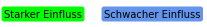
\includegraphics[]{img/legend.png}\\
    Leave-One-Out\\
    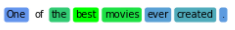
\includegraphics[]{img/first_ex_loo.png}\\
    Leave-N-Out\\
    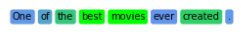
\includegraphics[]{img/first_ex_lno.png}
    \caption{Wie im Originalartikel wurde hier mit dem leave-n-out der Zusammenhang von \textit{best} und \textit{movies} besser gekennzeichnet. Im Gegensatz zum Originalartikel hingegen, wurde hier bei beiden das Wort \textit{created} als beeinflussend gekennzeichnet.}
    \label{fig:ex1}
\end{figure}

\begin{figure}[H]
    \centering
    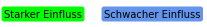
\includegraphics[]{img/legend.png}\\
    Leave-One-Out\\
    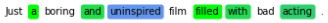
\includegraphics[]{img/sec_ex_loo.png}\\
    Leave-N-Out\\
    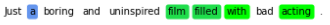
\includegraphics[]{img/sec_ex_lno.png}
    \caption{In diesem Beispiel werden viele Wörter als nicht beeinflussend gekennzeichnet. Die stark kronotierten Wörter \textit{boring} und \textit{uninspired} sowie \textit{bad} werden nicht beachtet. Die Ausgabestärke des Modells lag bei unter einem Prozent, wodurch erkennbar wird, dass hier das Modell sich nicht sicher ist wie es den Satz überhaupt einzuschätzen hat.}
    \label{fig:ex2}
\end{figure}

\begin{figure}[H]
    \centering
    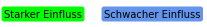
\includegraphics[]{img/legend.png}\\
    Leave-One-Out\\
    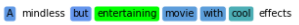
\includegraphics[]{img/third_ex_loo.png}\\
    Leave-N-Out\\
    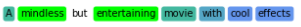
\includegraphics[]{img/third_ex_lno.png}
    \caption{Auch in diesem Beispiel findet sich eine Übereinstimmung zum Originalartikel. \textit{mindless} wird hier mit \textit{entertaining} stärker in Beziehung gesetzt.}
    \label{fig:ex3}
\end{figure}

\begin{figure}[H]
    \centering
    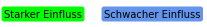
\includegraphics[]{img/legend.png}\\
    Leave-One-Out\\
    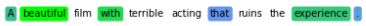
\includegraphics[]{img/fourth_ex_loo.png}\\
    Leave-N-Out\\
    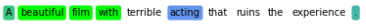
\includegraphics[]{img/fourth_ex_lno.png}
    \caption{Dieses Beispiel bietet gar keine Übereinstimmung mit dem Originalartikel. \textit{terrible} und \textit{ruins} werden gar nicht in Betracht gezogen. Aber auch hier ist das Modell der Fehler. Es klassifiziert bei diesem Beispiel das falsche Label.}
    \label{fig:ex4}
\end{figure}

Wie in den Abbildungen \ref{fig:ex1} bis \ref{fig:ex4} zu sehen ist, sind die Experimente zweigeteilt. Bei denen wo das
Klassifikationsmodell richtig liegt lässt sich auch die spätere Visualisierung des Originalartikes replizieren.
Jene Experimente wo das Modell schon im Vorhinein scheitert, haben auch eine schlechte Visualisierung.
Wie zuvor schon erwähnt, werden beim Visualisierungsprozess all die Wörter entfernt, welche nicht zur
Klassifikationbeitragen, also welche bei Entfernung die Ausgabestärke zum geschätzen Label verringern.
Schätzt das Modell nun also ein positives Label ob wohl es in wahrheit negativ ist, werden Wörter, die auf diese
Negativität hindeuten natürlich entfernt. Beim Weglassen wird das Dokument an sich positiver, wodurch die Wörter
scheinbar nichts zur Klassifikation beitragen und somit wegfallen.
Diese Tatsachen ergeben sich für alle stark, falsch klassifizierten Dokumente.

\begin{figure}[H]
    \centering
    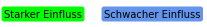
\includegraphics[]{img/legend.png}\\
    Leave-One-Out\\
    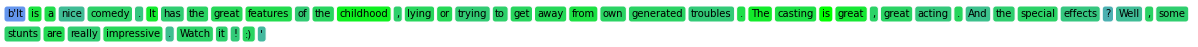
\includegraphics[width=\linewidth]{img/new_ex1_loo.png}\\
    Leave-N-Out\\
    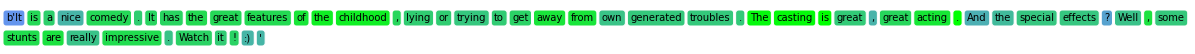
\includegraphics[width=\linewidth]{img/new_ex1_lno.png}
    \caption{Verlgeich längerer Texte. Veränderte Einflüsse fallen hier nur in Nuancen auf.}
    \label{fig:ex5}
\end{figure}

Bei längeren Texten fallen die veränderten Zusammenhänge nicht sofort auf.

\end{document}
